\chapter{Hamilton's mechanics}
\section{Hamilton's equations}
Now let's recap what we established with the differente pictures of classical mechanics that we discussed until now.
\begin{itemize}
    \item \eleref\;are a set of $n$ differential equations of $2^\circ$ order with $2n$ initial conditions
    \item When a coordinate is cyclic then: \begin{equation}
        p_{\alpha} = \pdv{\lagr}{\dot{q}_{\alpha}}\;\text{is conserved}
    \end{equation}
    but $p_{\alpha}$ is not a quantity of the Lagrangian
    \item even if $p_\alpha$ is conserved we still have $\dot{q}_{\alpha}$ as an ``extra'' term in the Lagrangian
\end{itemize}
We want to use a space differente from the configuration space in order to get rid of a useless term when a coordinate is cyclic. We then introduce a new concept.
\begin{definition}{Phase space}
  Phase space is a $2n$-dimensional space in which each point represents the \underline{state} of the system $\{q_{\alpha},p_{\alpha}\}$.
\end{definition}
Here are the fundamental differences between Lagrange formulation and Hamilton formulation of classical mechanics:
\begin{table}[H]
    \centering
    \begin{tabular}{lll}
        \underline{Lagrange} & $\longrightarrow$ &\underline{Hamilton}\\[8pt]
        $\lagr=\lagr(q_{\alpha},\dot{q}_{\alpha},t)$ & &$\hamfun=\hamfun(q_{\alpha},p_{\alpha},t)$\\[8pt]
        Configuration space & &Phase space\\[8pt]
        $n$ dimensions & &$2n$ dimensions
    \end{tabular}
\end{table}
Since we want to find a new function related to the Lagrangian that contains $p_{\alpha}$ as a variable instead of $\dot{q}_{\alpha}$, we need to introduce a certain type of transformation.\\
\textbf{Legendre transformations} are able to write a function $f(x,y)$ as a function $g(u,y)$ where:
\begin{equation}
    \dd{f} = \underbrace{\pdv{f}{x}}_u \dd{x} + \underbrace{\pdv{f}{y}}_v \dd{y} = u\dd{x} + v\dd{y}
\end{equation}
From this first relation we can work on the term $u\dd{x}$:
\begin{equation}
    \dd{(ux)} = u\dd{x} + x\dd{u} \Rightarrow u\dd{x} = \dd{(ux)} - x\dd{u}
\end{equation}
Then it is easy to see that a function $g = f-ux$ satisfies our conditions, and so we have:
\begin{equation}
    \dd{g} = \dd{(f-ux)} = - x\dd{u} + v\dd{y} \Rightarrow \begin{cases}
        \partial_{u} g = -x\\
        \partial_{y} g = v
    \end{cases}
\end{equation}
Let's try to apply Légendre transformations to the Lagrangian:
\begin{equation}
    \dd{\lagr} = \bigsum_{\alpha} \pdv{\lagr}{q_{\alpha}}\dd{q_{\alpha}} + \bigsum_{\alpha} \underbrace{\pdv{\lagr}{\dot{q}_{\alpha}}}_{p_{\alpha}}\dd{\dot{q}_{\alpha}} + \pdv{\lagr}{t}\dd{t}
\end{equation}
We then applied Légendre transformations to $\lagr$:
\begin{equation} \label{e:legendre_hamilton}
    \dd{\brackets{\lagr - \bigsum_{\alpha} p_{\alpha}\dot{q}_{\alpha}}} = \bigsum_{\alpha} \pdv{\lagr}{q_{\alpha}}\dd{q_{\alpha}} - \bigsum_{\alpha} \dot{q}_{\alpha}\dd{p_{\alpha}} + \pdv{\lagr}{t}\dd{t}
\end{equation}
And so if we define a function $\hamfun$ called \textbf{Hamiltonian} (or Hamilton function):
\begin{equation}
    \hamfun \defineeq \bigsum_{\alpha} p_{\alpha}\dot{q}_{\alpha} -\lagr
\end{equation}
Then \eqref{e:legendre_hamilton} becomes:
\begin{equation}
    \begin{split}
        -\dd{\hamfun} = \bigsum_{\alpha} \underbrace{\pdv{\lagr}{q_{\alpha}}}_{\dot{p}_{\alpha}}\dd{q_{\alpha}} - \bigsum_{\alpha} \dot{q}_{\alpha}\dd{p_{\alpha}} + \pdv{\lagr}{t}\dd{t}\\
        \dd{\hamfun} = -\bigsum_{\alpha} \dot{p}_{\alpha}\dd{q_{\alpha}} + \bigsum_{\alpha} \dot{q}_{\alpha}\dd{p_{\alpha}} - \pdv{\lagr}{t}\dd{t}\\
    \end{split}
\end{equation}
But also it is genrally true that:
\begin{equation}
    \dd{\hamfun} = \bigsum_{\alpha} \pdv{\hamfun}{q_{\alpha}}\dd{q_{\alpha}} + \bigsum_{\alpha} \pdv{\hamfun}{p_{\alpha}}\dd{p_{\alpha}} + \pdv{\hamfun}{t}\dd{t}
\end{equation}
The two equations must be equal so we get \textbf{Hamilton's canonical equations}:
\begin{equation} \label{hamilton_equations}
    \boxed{
    \begin{aligned}
        \pdv{\hamfun}{q_{\alpha}} &= -\dot{p}_{\alpha}\\
        \pdv{\hamfun}{p_{\alpha}} &=\;\;\;\dot{q}_{\alpha}\\
        \pdv{\hamfun}{t} &= -\pdv{\lagr}{t}
    \end{aligned}}
\end{equation}
This is a system of $2n (+1)$ equations, but they are first order ODEs so we have $2n$ initial conditions as in \lagrangeref. With this formulation we have one important advantage: if $q_j$ is cyclic then $\dot{p} = 0$, and we don't need to solve one of the differential equations.
This means that we only need $2n-1$ initial conditions. Same goes for any other cyclic coordinate, and so we have $2n-p$ initial conditions with $p$ being the number of cyclic coordinates.\\
Now let's remember the definition of the energy function:
\begin{equation}
    h = \bigsum_{\alpha}\underbrace{\pdv{\lagr}{q_{\alpha}}}_{p_{\alpha}}\dot{q}_{\alpha} - \lagr
\end{equation}
So we can say that the only difference between the energy function $h$ and the Hamiltonian $\hamfun$ is the fact that the first lives in the configuration space, the latter instead lives in the phase space.
To further convince ourselves of this fact we can evaluate the total derivative of $\hamfun$ over time:
\begin{equation}
    \begin{split}
        \dv{\hamfun}{t} &= \bigsum_{\alpha}\underbrace{\pdv{\hamfun}{q_{\alpha}}}_{-\dot{p}_{\alpha}}\dot{q}_{\alpha} + \bigsum_{\alpha}\underbrace{\pdv{\hamfun}{p_{\alpha}}}_{\dot{q}_{\alpha}}\dot{p}_{\alpha} + \pdv{\hamfun}{t} \\
        \dv{\hamfun}{t} &= \pdv{\hamfun}{t} = -\pdv{\lagr}{t}
    \end{split}
\end{equation}
So we get that $\hamfun$ will be the energy and/or will be conserved in the same situations of the energy function.
\section{Hamilton's equations through Hamilton's principle}
To derive \hamiltonref\;we can also exploit \hpquotemath\;starting from:
\begin{equation}
    \action = \int_{t_1}^{t_2}\lagr \dd{t}
\end{equation}
Using the same definition for $\hamfun$ that we previously used:
\begin{equation}
    \hamfun = \bigsum_{\alpha}p_{\alpha}\dot{q}_{\alpha} - \lagr
\end{equation}
We get:
\begin{equation} \label{e:deltaS_hamilton}
    \delta \action = \int_{t_1}^{t_2}\bbrackets{\bigsum_{\alpha}\delta p_{\alpha}\dot{q}_{\alpha} + \bigsum_{\alpha} p_{\alpha} \underbrace{\delta \dot{q}_{\alpha}}_{\frac{\dd{}}{\dd{t}}\delta q_{\alpha}} - \bigsum_{\alpha} \pdv{\hamfun}{q_{\alpha}} \delta q_{\alpha}- \bigsum_{\alpha} \pdv{\hamfun}{p_{\alpha}} \delta p_{\alpha}} \dd{t}
\end{equation}
We apply the product rule on the second member:
\begin{equation}
    \bigsum_{\alpha} p_{\alpha} \dv{}{t}\delta q_{\alpha} = \bigsum_{\alpha} \bigg[ \dv{}{t} \brackets{p_{\alpha} \delta q_{\alpha}} -  \delta q_{\alpha}\dv{}{t}p_{\alpha}\bigg]
\end{equation}
Integrating the first term we get:
\begin{equation}
    \int_{t_1}^{t_2} \bigsum_{\alpha} \dv{}{t} \brackets{p_{\alpha} \delta q_{\alpha}} \dd{t} = \bigsum_{\alpha} p_{\alpha} \delta q_{\alpha} \bigg|_{t_1}^{t_2} = 0
\end{equation}
This is zero because in \hpquotemath\;we assumed that the virtual displacement at the extreme points is zero. So we can rewrite \eqref{e:deltaS_hamilton} putting in evidence the common terms:
\begin{equation}
    \begin{split}
        \delta \action &= \int_{t_1}^{t_2}\bbrackets{\bigsum_{\alpha}\delta p_{\alpha}\dot{q}_{\alpha} - \bigsum_{\alpha} \delta q_{\alpha}\dot{p}_{\alpha} - \bigsum_{\alpha} \pdv{\hamfun}{q_{\alpha}} \delta q_{\alpha}- \bigsum_{\alpha} \pdv{\hamfun}{p_{\alpha}} \delta p_{\alpha}} \dd{t} \\
        \delta \action &= \int_{t_1}^{t_2}\bbrackets{\bigsum_{\alpha}\bigg[\dot{q}_{\alpha} - \pdv{\hamfun}{p_{\alpha}}\bigg] \delta p_{\alpha} - \bigsum_{\alpha} \bigg[\dot{p}_{\alpha} + \pdv{\hamfun}{q_{\alpha}} \bigg]\delta q_{\alpha}} \dd{t} = 0
    \end{split}
\end{equation}
Since all the terms are independent by construction all the brackets must be zero. In this way we get the same set of equation as we did before.
\section{Poisson brackets}
In the context of Hamilton's mechanics we can introduce the notion of the \textbf{Poisson brackets}.\\
Consider two functions $f,g$ in the phase space:
\begin{equation}
    \begin{cases}
        f = f(q_{\alpha},p_{\alpha},t)\\
        g = g(q_{\alpha},p_{\alpha},t)
    \end{cases}
\end{equation}
We define Poisson brackets as follows:
\begin{equation}
    \pb{f}{g} = \bigsum_{\alpha}\brackets{\pdv{f}{q_{\alpha}}\pdv{g}{p_\alpha} - \pdv{f}{p_{\alpha}}\pdv{g}{q_{\alpha}}}
\end{equation}
Notice that $\pb{f}{g}$ is still a function in the phase space.\\
Now we can give some \underline{properties} of the Poisson brackets:
\begin{enumerate}
    \item antisimmetry: \[\pb{f}{g} = - \pb{g}{f}\]
    \item bilinearity:
    \[\pb{\alpha f + \beta g}{h} = \alpha\pb{f}{h}+ \beta\pb{g}{h}\]
    \[\pb{h}{\alpha f + \beta g} = \alpha\pb{h}{f}+ \beta\pb{h}{g}\]
    \item Leibniz rule: \[\pb{f}{gh} = g\pb{f}{h} + \pb{f}{g}h\]
    \item Jacobi identity: \[\pb{f}{\pb{g}{h}} + \pb{h}{\pb{f}{g}} + \pb{g}{\pb{h}{f}} = 0\]
\end{enumerate}
Given this definition let's evaluate the total time derivative of a function $f$ in the phase space:
\begin{equation}
    \dv{f}{t} = \bigsum_{\alpha}\brackets{\pdv{f}{q_{\alpha}}\dot{q}_{\alpha} + \pdv{f}{p_{\alpha}}\dot{p}_{\alpha}} + \pdv{f}{t}
\end{equation}
Using \hamiltonref\;we can rewrite this as:
\begin{equation}
    \begin{split}
        \dv{f}{t} &= \bigsum_{\alpha}\brackets{\pdv{f}{q_{\alpha}}\pdv{\hamfun}{p_{\alpha}} - \pdv{f}{p_{\alpha}}\pdv{\hamfun}{q_{\alpha}}} + \pdv{f}{t}\\[8pt]
        \dv{f}{t} &= \pb{f}{\hamfun} + \pdv{f}{t}
    \end{split}
\end{equation}
And so we can get a new condition for any generic function $f$ to be a constant of motion:
\begin{equation}
    f\;\text{is conserved} \iff \dv{f}{t} = 0 \iff \pb{f}{\hamfun} = -\pdv{f}{t}
\end{equation}
Furter more if $f$ is independent of time the condition is:
\begin{equation}
    \pb{f}{\hamfun} = 0
\end{equation}
\section{Examples}
\subsection{Ex. 1}
Let us start with a simple example. Consider an unconstrained particle moving on a frictionless plane under the action of a potential $V(x,y)$. We have 2 degrees of freedom. We can simply choose cartesian coordinates and write the Lagrangian:
\begin{equation}
  \lagr = T - V = \dfrac{1}{2}m(\dot{x}^2+\dot{y}^2) - V(x,y)
\end{equation}
Now the conjugated momenta are:
\begin{equation}
  \begin{split}
    &p_x = m\dot{x} \\[8pt]
    &p_y = m\dot{y}
  \end{split}
\end{equation}
And so the Hamiltonian is:
\begin{equation}
  \begin{split}
    \hamfun &= p_x\dot{x} + p_y\dot{y} - \dfrac{1}{2}m(\dot{x}^2+\dot{y}^2) + V(x,y) =\\[8pt]
    &= m(\dot{x}^2+\dot{y}^2) - \dfrac{1}{2}m(\dot{x}^2+\dot{y}^2) + V(x,y) = \dfrac{\vec{p}^2}{2m} + V(x,y)
  \end{split}
\end{equation}
Here $T$ is a quadratic function of the velocities and $V$ does not depend on the velocities, hence $\hamfun = E$ as expected. The first two \hamiltonref\;are:
\begin{equation}
  \begin{split}
    \dot{x} = \pdv{\hamfun}{p_x} = \dfrac{p_x}{m} \\[8pt]
    \dot{y} = \pdv{\hamfun}{p_y} = \dfrac{p_y}{m}
  \end{split}
\end{equation}
Those are already known. We also have that:
\begin{equation}
  \begin{split}
    \dot{p}_x = -\pdv{\hamfun}{x} = -\pdv{V}{x} \\[8pt]
    \dot{p}_y = -\pdv{\hamfun}{y} = -\pdv{V}{y}
  \end{split}
\end{equation}
And so:
\begin{equation}
  \dot{\vec{p}} = -\grad{V} = \vec{F}
\end{equation}
Again we find something that is not new.\\
\subsection{Ex. 2}
\begin{figure}[H]
  \centering
  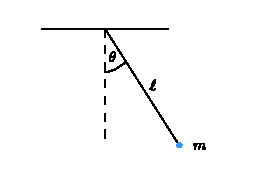
\includegraphics[width=0.5\linewidth]{res/svg/simple_pendulum.drawio}
  \caption{Simple pendulum}
\end{figure}
Now we can discuss the problem of a simple pendulum in the Hamilton formalism. We have a mass $m$ attached to a thin massless rod of length $\ell$. The constraint given by the rod is holonomic and scleronomic:
\begin{equation}
  x^2+y^2-\ell^2 = 0
\end{equation}
We have only one independent coordinate. Let us choose the angle $\theta$. We have that:
\begin{equation}
  \begin{split}
    &x = \ell \cos \theta \implies \dot{x} = - \ell \dot{\theta}\sin \theta \\[8pt]
    &y = \ell \sin \theta \implies \dot{y} = \ell \dot{\theta}\cos \theta
  \end{split}
\end{equation}
The potential is just given by the gravitational potential, which in the reference frame that we fixed is:
\begin{equation}
  V = -mgy = -mg \ell \cos \theta
\end{equation}
The Lagrangian is:
\begin{equation}
  \lagr = \dfrac{1}{2}m\ell^2\dot{\theta}^2 + mg \ell \cos \theta
\end{equation}
The conjugated momenta is:
\begin{equation}
  p_{\theta} = \pdv{\lagr}{\dot{\theta}} = m\ell^2\dot{\theta} = L_z
\end{equation}
And so:
\begin{equation}
  \dot{\theta} = \dfrac{L_z}{m\ell^2}
\end{equation}
The Hamiltonian is:
\begin{equation}
  \hamfun = p_{\theta}\dot{\theta} - \lagr = L_z\dot{\theta} - \dfrac{1}{2}\dfrac{L_z^2}{m\ell^2} - mg \ell \cos \theta = \dfrac{p_{\theta}^2}{2m\ell^2} - mg \ell \cos \theta
\end{equation}
The first \hamiltonref\;gives:
\begin{equation}
  \dot{\theta} = \pdv{\hamfun}{p_{\theta}} = \dfrac{L_z}{m\ell^2}
\end{equation}
Which is already known. The second one gives:
\begin{equation}
  \dot{p}_\theta = -\pdv{\hamfun}{\theta} = - mg \ell \sin \theta
\end{equation}
And so we have:
\begin{equation}
  \begin{split}
    &\dv{}{t}\brackets{m\ell^2\dot{\theta}} = - mg \ell \sin \theta \\[8pt]
    &\boxed{\ddot{\theta} = - \dfrac{g}{\ell} \sin \theta}
  \end{split}
\end{equation}
This is indeed the known equation for the pendulum.\\
\subsection{Ex. 3}
\begin{figure}[H]
  \centering
  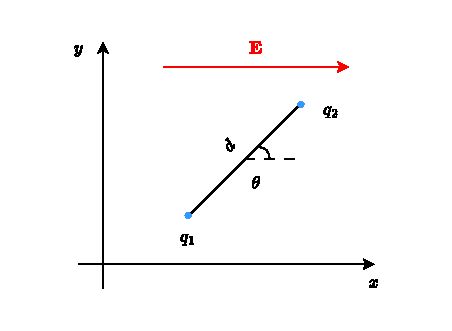
\includegraphics[width=0.5\linewidth]{res/svg/dipole.drawio}
\end{figure}
Now let us take a system made of two charges $q_1$ and $q_2$ of equal mass, with a bar with negligible mass that fixes the distance $d$. Imagine there is an electrostatic field acting on the particles. The motion of the particles is happening on a plane so we have 3 generalized coordinates. We can take the coordinates of the centre of mass $(X, Y)$ and the angle of the bar. We can split the contribution of the kinetic energy with the contribution of the centre of mass and the rotation around the centre of mass:
\begin{equation}
  T = T_{CM} + T' = \dfrac{1}{2}M(\dot{X}^2+\dot{Y}^2) + \dfrac{1}{2}I\dot{\theta}^2
\end{equation}
Now we know $M = 2m$ and $I = 2m\brackets{\dfrac{d}{2}}^2 = \dfrac{1}{2}md^2$. The kinetic energy is thus:
\begin{equation}
  T = m(\dot{X}^2+\dot{Y}^2) + \dfrac{1}{4}md^2\dot{\theta}^2
\end{equation}
Now we could in theory use three different approaches:
\begin{itemize}
  \item Use Lagrange equations
  \item Define a potential and use \eleref
  \item Find the Hamiltonian and use \hamiltonref
\end{itemize}
In this case we use the third method under the assumption that $\vec{E} = (E(x), 0, 0)$. Thus, the electric field is only given by the x component of a potential:
\begin{equation}
  E(x) = -\pdv{\potE}{x}
\end{equation}
The gravitational potential is negligible and so:
\begin{equation}
  V = q_1\potE(x_1) + q_2\potE(x_2)
\end{equation}
Which expressed in terms of the generalized coordinates becomes:
\begin{equation}
  V = q_1\potE \brackets{X - \dfrac{d}{2}\cos\theta} + q_2\potE \brackets{X + \dfrac{d}{2}\cos\theta}
\end{equation}
The Lagrangian is:
\begin{equation}
  \lagr = T - V = m(\dot{X}^2+\dot{Y}^2) + \dfrac{1}{4}md^2\dot{\theta}^2 - q_1\potE \brackets{X - \dfrac{d}{2}\cos\theta} - q_2\potE \brackets{X + \dfrac{d}{2}\cos\theta}
\end{equation}
We should also account for a interaction potential but since the distance is fixed this term would be constant and thus the Lagrangian can be defined without it. The Lagrangian does not depend on time thus:
\begin{equation}
  \pdv{\hamfun}{t} = - \pdv{\lagr}{t} = 0 \implies \dv{\hamfun}{t} = 0
\end{equation}
And so the Hamiltonian is a constant of the motion. Also transformation equations do not depend on time and the potential does not depend on the velocities thus $\hamfun = E$. So the Hamiltonian is the energy and it is conserved. Now we find the conjugated momenta:
\begin{equation}
  \begin{split}
    &p_X = \pdv{\lagr}{\dot{X}} = 2m\dot{X} \\[8pt]
    &p_Y = \pdv{\lagr}{\dot{Y}} = 2m\dot{Y} \\[8pt]
    &p_\theta = \pdv{\lagr}{\dot{\theta}} = \dfrac{1}{2}md^2\dot{\theta} = L_z \\[8pt]
  \end{split}
\end{equation}
The Hamiltonian will be:
\begin{equation}
  \begin{split}
    \hamfun &= 2m\dot{X}^2 + 2m\dot{Y}^2+ \dfrac{1}{2}md^2\dot{\theta}^2 - m(\dot{X}^2+\dot{Y}^2) - \dfrac{1}{4}md^2\dot{\theta}^2 + \\[8pt]
    &+ q_1\potE \brackets{X - \dfrac{d}{2}\cos\theta} + q_2\potE \brackets{X + \dfrac{d}{2}\cos\theta} = \\[8pt]
    &= m\brackets{\dot{X}^2 + \dot{Y}^2} + \dfrac{L_z^2}{md^2} + q_1\potE \brackets{X - \dfrac{d}{2}\cos\theta} + q_2\potE \brackets{X + \dfrac{d}{2}\cos\theta}
  \end{split}
\end{equation}
Now the interesting \hamiltonref\;are the ones who give the $\dot{p}_{\alpha}$ since we already know the $\dot{q}_{\alpha}$ in terms of the momenta from the Lagrangian part. We have that:
\begin{equation}
  \begin{split}
    &\dot{p}_X = -\pdv{\hamfun}{X} = - q_1 \pdv{\potE}{X} - q_2 \pdv{\potE}{X} = q_1E(x_1) + q_2E(x_2) \\[8pt]
    &\dot{p}_Y = -\pdv{\hamfun}{Y} = 0 \\[8pt]
    &\dot{p}_\theta = -\pdv{\hamfun}{\theta} = - q_1 \pdv{\potE}{\theta} - q_2 \pdv{\potE}{\theta} = - q_1 \pdv{\potE}{x_1}\pdv{x_1}{\theta} - q_2 \pdv{\potE}{x_2}\pdv{x_2}{\theta} = \\[8pt]
    &= q_1E(x_1)\dfrac{d}{2}\sin \theta - q_2E(x_2)\dfrac{d}{2}\sin \theta
  \end{split}
\end{equation}
And so $\dot{p}_X$ is the total force and $\dot{p}_{\theta}$ is the total torque. Now consider the case where the two charges are equal but have opposite sign ($q_1 = -q$, $q_2 = q$):
\begin{equation}
  \dot{p}_X = q \brackets{E(x_2) - E(x_1)}\\[8pt]
\end{equation}
If the field is uniform $E(x_2) = E(x_1) = E \implies \vec{F} = 0$, but we still have torque:
\begin{equation}
  \dv{L_z}{t} = -q\dfrac{d}{2}\sin \theta \brackets{E(x_1) + E(x_2)} = -\underbrace{qd}_p E\sin \theta
\end{equation}
And so:
\begin{equation}
  \dv{L_z}{t} = -\brackets{\vec{p} \cross \vec{E}}_z
\end{equation}
Where $\vec{p}$ is the dipole vector.
\subsection{Ex. 4}
\begin{figure}[H]
  \centering
  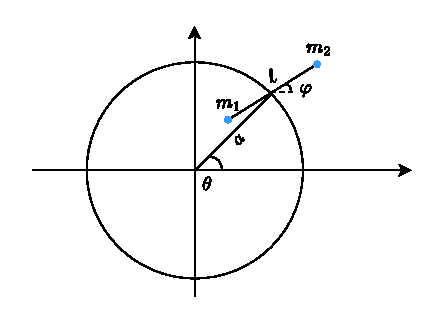
\includegraphics[width=0.7\linewidth]{res/svg/rail_and_bar.drawio}
\end{figure}
A massless bar of length $\ell$ with two bodies $m_1$, $m_2$ is attached in the centre of mass to a system composed of a vertical rail of radius $a$. The system is under the action of the gravitational potential. We have $2$ masses so we start from $3N = 6$ cartesian coordinates, but the motion is constrained on the vertical plane and we also have two constraints which are the bar and the rail so the number of independent coordinates is $n=2$. We can simply use the angles $\theta$ and $\varphi$ to describe the system. The coordiantes of the centre of mass are:
\begin{equation}
  \begin{split}
    X &= a\cos\theta \\[8pt]
    Y &= a\sin\theta
  \end{split}
\end{equation}
If the masses are equal $m_1 = m_2 = m$ then their coordiantes are:
\begin{equation}
  \begin{split}
    &x_1 = X - \dfrac{\ell}{2}\cos\varphi = a\cos\theta - \dfrac{\ell}{2}\cos\varphi \\[8pt]
    &y_1 = Y - \dfrac{\ell}{2}\sin\varphi = a\sin\theta - \dfrac{\ell}{2}\sin\varphi \\[8pt]
    &x_2 = X + \dfrac{\ell}{2}\cos\varphi = a\cos\theta + \dfrac{\ell}{2}\cos\varphi \\[8pt]
    &y_2 = Y + \dfrac{\ell}{2}\sin\varphi = a\sin\theta + \dfrac{\ell}{2}\sin\varphi \\[8pt]
  \end{split}
\end{equation}
The transformation equations do not depend on time so the kinetic energy will be a quadratic function of the velocities. We have that:
\begin{equation}
  \begin{split}
    &\dot{x}_1 = -a\dot{\theta}\sin\theta + \dfrac{\ell}{2}\dot{\varphi}\sin\varphi \\[8pt]
    &\dot{y}_1 = a\dot{\theta}\cos\theta - \dfrac{\ell}{2}\dot{\varphi}\cos\varphi \\[8pt]
    &\dot{x}_2 = -a\dot{\theta}\sin\theta - \dfrac{\ell}{2}\dot{\varphi}\sin\varphi \\[8pt]
    &\dot{y}_2 = a\dot{\theta}\cos\theta + \dfrac{\ell}{2}\dot{\varphi}\cos\varphi \\[8pt]
  \end{split}
\end{equation}
And so the kinetic energy will be:
\begin{equation}
  T = \frac{1}{2}m\left(\dot{x}_1^2 + \dot{y}_1^2 + \dot{x}_2^2 + \dot{y}_2^2\right) = m a^2 \dot{\theta}^2 + \frac{1}{4} m \ell^2 \dot{\varphi}^2
\end{equation}
We could have gotten this just by applying König's theorem:
\begin{equation}
  T = T' + T_{CM} = m a^2 \dot{\theta}^2 + \frac{1}{4} m \ell^2 \dot{\varphi}^2
\end{equation}
The potential is simply:
\begin{equation}
  V = mg\brackets{y_1 + y_2} = mg\brackets{a\sin\theta - \cancel{\dfrac{\ell}{2}\sin\varphi} + a\sin\theta + \cancel{\dfrac{\ell}{2}\sin\varphi}} = 2mga\sin\theta
\end{equation}
And so the Lagrangian is:
\begin{equation}
  \lagr = T - V = m a^2 \dot{\theta}^2 + \frac{1}{4} m \ell^2 \dot{\varphi}^2 - 2mga\sin\theta
\end{equation}
Thus the two conjugate momenta are:
\begin{equation}
  \begin{split}
    p_{\theta} = \pdv{\lagr}{\dot{\theta}} = 2m a^2 \dot{\theta} \\[8pt]
    p_{\varphi} = \pdv{\lagr}{\dot{\varphi}} = \dfrac{1}{2} m \ell^2 \dot{\varphi}
  \end{split}
\end{equation}
We can notice that $p_{\varphi}$ is constant since $\varphi$ is a cyclic coordinate. We can now find the Hamiltonian:
\begin{equation}
  \hamfun = p_{\theta}\dot{\theta} + p_{\varphi}\dot{\varphi} - \lagr = \frac{p_{\theta}^2}{4ma^2} + \frac{p_{\varphi}^2}{m\ell^2} + 2mga\sin\theta
\end{equation}
We only need to solve one Hamilton equation since we already know the relations between the coordinates and the momenta and we also knwo that $\dot{p}_{\varphi} = 0$ so we have:
\begin{equation}
  \dot{p}_{\theta} = -\pdv{\hamfun}{\theta} = -2mga\cos\theta
\end{equation}
The quantity $2mga\cos\theta$ is actually the $z$ component of the torque $\tau_z$ and this means that the system is rotating without a constant angular momentum under the action of gravity, which is what we expect from the setup we have. The equation above also gives us:
\begin{equation}
  \begin{split}
    &2m a^2 \ddot{\theta} = -2mga\cos\theta \\[8pt]
    &\ddot{\theta} + \dfrac{g}{a}\cos\theta = 0
  \end{split}
\end{equation}
\begin{figure}[H]
  \centering
  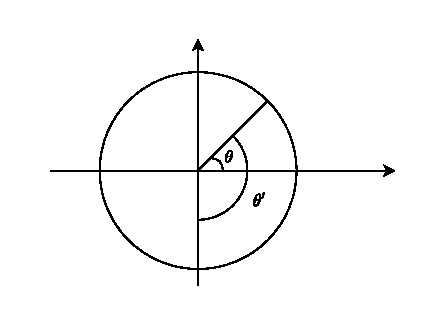
\includegraphics[width=0.5\linewidth]{res/svg/theta_prime.drawio}
\end{figure}
Now if we use the angle $\theta' = \theta + \dfrac{\pi}{2}$ to describe the system we end up with:
\begin{equation}
  \ddot{\theta'} + \dfrac{g}{a}\sin\theta' = 0
\end{equation}
Which is the equation of motion of a pendulum, so the bar is rotating with constant angular momentum around the centre of mass and the centre of mass is moving periodically on the rail.
